\documentclass[Royal,times,sageh]{sagej}

\usepackage{moreverb,url,natbib, multirow, tabularx}
\usepackage[colorlinks,bookmarksopen,bookmarksnumbered,citecolor=red,urlcolor=red]{hyperref}





\begin{document}

\title{Missing the Point: Non-Convergence in Iterative Imputation Algorithms}

\runninghead{Oberman}

\author{H. I. Oberman\affilnum{1}}

\affiliation{\affilnum{1}{Department of Methodology and Statistics, Utrecht University, Utrecht, The Netherlands}}

\corrauth{Hanne Oberman, Sjoerd Groenman building, Utrecht Science Park, Utrecht, The Netherlands.}

\email{\href{mailto:h.i.oberman@uu.nl}{\nolinkurl{h.i.oberman@uu.nl}}}

\begin{abstract}
Iterative imputation is a popular tool to accommodate missing data. While it is widely accepted that valid inferences can be obtained with this technique, these inferences all rely on algorithmic convergence. There is no consensus on how to evaluate the convergence properties of the method. This paper provides insight into identifying non-convergence of iterative imputation algorithms. We conclude that in the case of drawing inference from incomplete data, convergence of the iterative imputation algorithm is often a convenience but not a necessity.
\end{abstract}

\keywords{missing data, iterative imputation, non-convergence, mice}

\maketitle

\hypertarget{introduction}{%
\section{Introduction}\label{introduction}}

Anyone who analyzes person-data may run into a missing data problem. Missing data is not only ubiquitous across science, but treating it can also be a tedious task. If a dataset contains just one incomplete observation, calculations are not defined, and statistical models cannot be fitted to the data. To circumvent this, many statistical packages employ list-wise deletion by default (i.e., ignoring incomplete observations). Unfortunately, this \emph{ad hoc} solution may yield invalid results \citep{buur18}. An alternative is to apply imputation. With imputation, we `fill in' the missing values in an incomplete dataset. Subsequently, the model of scientific interest can be fitted to the completed dataset. By repeating this process several times, a distribution of plausible results may be obtained, which reflects the uncertainty in the data due to missingness. This technique is known as `multiple imputation' \citep[MI;][]{rubin76}. MI has proven to be a powerful technique to draw valid inferences from incomplete data under many circumstances \citep{buur18}.

Figure \ref{fig:diagram} provides an overview of the steps involved with MI. The missing part \(y_{\rm mis}\) of an incomplete dataset is imputed \(m\) times. This creates \(m\) sets of imputed data \(\dot y_{\rm imp, \ell}\), where \(\ell = 1, 2, ..., m\). The imputed data is then combined with the observed data \(y_{\rm obs}\) to create \(m\) completed datasets. On each of these datasets the analysis of scientific interest is performed to estimate \(Q\): the quantity of scientific interest (e.g., a regression coefficient). Since \(Q\) is estimated on each completed dataset, \(m\) separate \(\hat{Q}_\ell\)-values are obtained. Finally, the \(\hat{Q}_\ell\)-values are combined into a single pooled estimate \(\bar{Q}\). The premise of multiple imputation is that \(\bar{Q}\) is an unbiased and confidence-valid estimate of the true---but unobserved---scientific estimand \(Q\) \citep{rubin96}.

\begin{figure}

{\centering 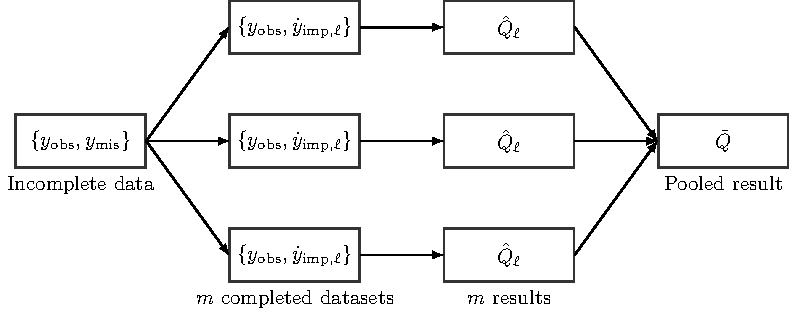
\includegraphics[width=\linewidth]{../Figures/DiagramMI} 

}

\caption{Scheme of the main steps in multiple imputation---from an incomplete dataset, to $m=3$ multiply imputed datasets, to $m=3$ estimated quantities of scientific interest $\hat{Q}$s, to a single pooled estimate $\bar{Q}$.}\label{fig:diagram}
\end{figure}

A popular method to obtain imputations \(\dot y_{\rm imp, \ell}\) is to use the `Multiple Imputation by Chained Equations' algorithm, shorthand `MICE'\citep{mice}. With MICE, imputed values are drawn from the posterior predictive distribution of the missing values \(y_{\rm mis}\). The algorithm is named after the iterative algorithmic procedure by which imputed values are generated: a multivariate distribution is obtained by iterating over a sequence of univariate imputations. The iterative nature of algorithms like MICE introduces a potential threat to the validity of the imputations: What if the algorithm has not converged? Are the imputations then to be trusted? And can we rely on the inference obtained on the completed data?

These remain open questions, since the convergence properties of iterative imputation algorithms have not been systematically studied \citep{buur18}. There is no scientific consensus on how to evaluate the convergence of imputation algorithms \citep{taka17}. Moreover, the behavoir of such algorithms under certain default imputation models (e.g., `predictive mean matching') is an entirely open question \citep{murr18}. Therefore, algorithmic convergence should be monitored carefully, \textbf{but this is not straightforward}. Iterative imputation algorithms such as MICE are special cases of Markov chain Monte Carlo (MCMC) methods. In MCMC methods, convergence is not from a scalar to a point, but from one distribution to another. The values generated by the algorithm (e.g., imputed values) will vary even after convergence \citep{gelm13}. Since MCMC algorithms do not reach a unique point at which convergence is established, diagnostics may only identify signs of \emph{non}-convergence \citep{hoff09}. Several of such non-convergence diagnostics exist, but it is not known whether these are appropriate for iterative imputation algorithms.

In this paper, we study different methods for assessing non-convergence in iterative imputation algorithms. We define several diagnostics and evaluate how these diagnostics could be appropriate for iterative imputation applications. We then adress the impact of inducing non-convergence in iterative imputation algorithms through model-based simulation in \texttt{R} \citep{R}. The aim of the simulation study is to determine whether unbiased, confidence-valid inferences may be obtained if the algorithm has not (yet) converged. And additionally, to formulate an informed advice on when approxiamte convergence may be safely concluded. We will therefore assess the performance of different methods to identify non-convergence. We translate the results of the study into guidelines for applied researchers. \textbf{ADD that these guidelines may aid to draw valid inference from incomplete data?{]}} For reasons of brevity, we only focus on the iterative imputation algorithm implemented in the popular \texttt{mice} package \citep{mice} in \texttt{R} \citep{R}.

\hypertarget{some-notation}{%
\subsection{Some notation}\label{some-notation}}

Let \(y\) denote an \(n \times k\) matrix containing the data values on \(k\) variables for all \(n\) units in a sample. The data value of unit \(i\) (\(i = 1, 2, \dots, n\)) on variable \(j\) (\(j = 1, 2, \dots, k\)) may be either observed or missing. The number of units \(i\) with at least one missing value, divided by the total number of units \(n\), is called the missingness proportion \(p_{\rm mis}\) in dataset \(y\). The collection of observed data values in \(y\) is denoted by \(y_{\rm obs}\); the missing part of \(y\) is referred to as \(y_{\rm mis}\). For each datapoint in \(y_{\rm mis}\), we sample \(m \times T\) plausible values, where \(m\) is the number of imputations (\(\ell = 1, 2, \dots, m\)) and \(T\) is the number of iterations (\(t = 1, 2, \dots, T\)) in the imputation algorithm. The state space of the algorithm at a certain iteration \(t\) may be summarized by a scalar summary \(\theta\) (e.g., \textbf{the average of the imputed values}). The collection of \(\theta\)-values between the \textbf{initial value} (at \(t=1\)) and the final imputed value (at \(t=T\)) will be referred to as an `imputation chain'.

\hypertarget{algorithmic-non-convergence}{%
\section{Algorithmic non-convergence}\label{algorithmic-non-convergence}}

There are two requirements for convergence of iterative algorithms: mixing and stationarity \citep{gelm13}. In iterative imputation algorithms mixing implies that imputation chains intermingle nicely, and stationarity is characterized by \textbf{the absence of trending} within chains. If one of these two requirements is not met, there is non-convergence in the algorithm. Without mixing, chains may be `stuck' at a local optimum, instead of sampling imputed values from the entire predictive posterior distribution of the missing values. The distribution of imputed values then differs across imputations. This may cause under-estimation of the variance between chains, which results in spurious, invalid inferences. Without stationarity, there is trending within imputation chains. Trending implies that further iterations would yield a systematically lower or higher set of imputations. Iterative imputation algorithms that have not (yet) reached stationarity, may thus yield biased estimates.

To illustrate what non-mixing and non-stationarity looks like in iterative imputation algorithms, we reproduce an example from van Buuren \citeyearpar[\(\S\) 6.5.2]{buur18}. Figure \ref{fig:non-conv} displays two scenarios from the example. The graph on the left-hand side of the figure shows typical convergence of an iterative imputation algorithm. The right-hand side displays pathological non-convergence, induced by purposefully mis-specifying the imputation model. Each line portrays one imputation chain: scalar summary \(\theta\) plotted against the iteration number \(t\). The \(\theta\) in this example is the chain mean of a variable that we will call \(j\) (i.e., the average of the imputed values for \(j\) in each imputation \(\dot y_{\rm imp, \ell}\)). In the typical convergence scenario, the imputation chains intermingle nicely and there is little to no trending. In the non-convergence scenario, there is a lot of trending and some chains do not intermingle. Importantly, the chain means at the last iteration (the imputed value per imputation \(\ell\)) are very different between the two plots. The algorithm with the mis-specified model yields imputed values that are on average a factor two larger than those of the typically converged algorithm. Non-convergence thus influences the mean of \(j\) in \(\dot y_{\rm imp, \ell}\). This difference (presumably) translates to the \(m\) completed data estimates \(\hat{\mu}_{j,\ell}\), and consequently to the pooled estimate \(\bar{\mu}_j\). Ergo, non-convergence leads to biased estimates. This shows the importance of reaching converged states in iterative imputation algorithms.

\begin{figure}

{\centering 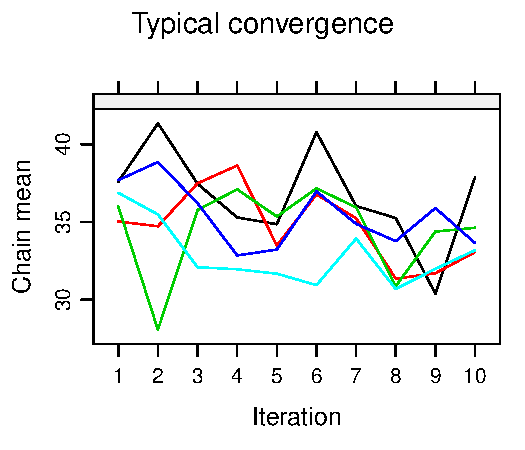
\includegraphics[width=.49\linewidth]{2.Manuscript_files/figure-latex/non-conv-1} 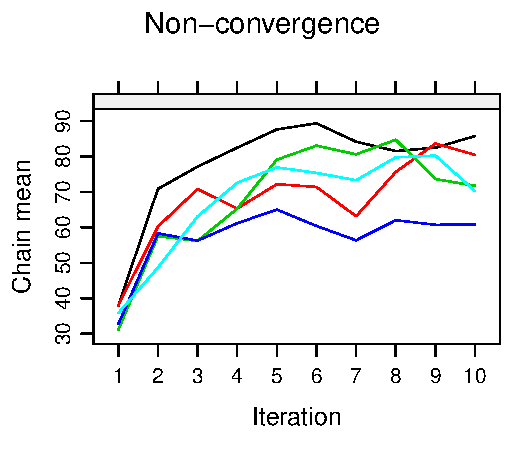
\includegraphics[width=.49\linewidth]{2.Manuscript_files/figure-latex/non-conv-2} 

}

\caption{Typical convergence versus pathological non-convergence. Please note that this is the same data with a different imputation model, leading to different imputations (e.g., see the units on the y-axis).}\label{fig:non-conv}
\end{figure}

\textbf{{[}MERGE with sections below{]}} Currently, the recommended practice for evaluating the convergence of the MICE algorithm is through visual inspection. After running the imputation algorithm for a certain number of iterations, its convergence is monitiored by plotting a scalar summary of the state space of the algorithm \(\theta\) against the iteration number. Typically, the \(\theta\)s under evaluation are chain means and variances---the average and the variance of the imputed values per imputation. Monitoring convergence by inspecting traceplots of these \(\theta\)s may be undesirable for several reasons: 1) it may be challenging to the untrained eye, and 2) only severely pathological cases of non-convergence may be diagnosed \citep[\(\S\) 6.5.2]{buur18} and, 3) there is not an objective measure that quantifies convergence.

\textbf{{[}MERGE with section above and below{]}} Inspecting non-convergence through traceplots of chain means and chain variances may be insufficient because they are univariate summaries of the state space of the algorithm, while MICE is not only concerned with a single column, but the entire multivariate distribution of \(y_{\rm imp}\). Ideally, a multivariate \(\theta\) should be monitored. A suggestion by \citet{buur18} for a multivariate \(\theta\) to monitor is the quantity of scientific interest \(Q\) (e.g., a regression coefficient), which usually is multivariate in nature. Implementing this, however, might be somewhat too technical for empirical researchers. Moreover, this scalar summary is not model-independent, i.e., it only applies to one model of scientific interest. Yet, one of the advantages of MI is that the missing data problem and scientific problem are solved independently. On these grounds, such a \(\theta\) can be considered insufficient too. Van Buuren \citeyearpar[\(\S\) 4.5.2]{buur18} also proposed multivariable evaluation of the MICE algorithm through eigenvalue decomposition, building on the work of \citet{mack03}. Eigenvalues of a variance-covariance matrix are a measure of the data's total covariance. Such a \(\theta\) would be a model-independent, multivariate scalar summary to monitor, but it is not implemented in \texttt{mice}.

\textbf{{[}MERGE with sections above{]}} Convergence has historically been inspected visually, by monitoring the imputation algorithm over iterations. This is typically done through traceplots. In a traceplot, the iteration number is plotted against a certain \(\theta\). \(\theta\)s are scalar summaries of the state space of the algorithm at a specific iteration. The default scalar summaries in \texttt{mice} are chain means and chain variances. Additionally, researchers may ``monitor some statistic of scientific interest'' \citep[\(\S\) 6.5.2]{buur18}. As \citet{buur18} describes, researchers can specify their quantity of scientific interest \(Q\) (e.g., a regression coefficient) as scalar summary \(\theta\). Such a user-defined scalar summary, however, may be somewhat advanced for empirical researchers. And moreover, it is not universal to all complete data problems. Focusing on the convergence of outcome parameters may influence the iterative imputation procedure in the sense that the model of evaluation favors the model of interest. The downside to these two approaches is that they either focus on the univariate state space, or primarily track the change over the iterations of a multivariate outcome conform the scientific model of interest. Ideally, one would like to evaluate a model-independent parameter that summarizes the multivariate nature of the data. Therefore, we propose a \(\theta\) that summarizes the multivariate state space of the algorithm, but is independent from the model of scientific interest. We propose \(\lambda_{1, \ell}\) as such a scalar summary. We define \(\lambda_{1, \ell}\) as the first eigenvalue of the variance-covariance matrix of the completed data. Let \(\lambda_{1, \ell} \geq \lambda_{2, \ell} \geq ... \geq \lambda_{j, \ell}\) be the eigenvalues of \(\Sigma_\ell\) in each of the \(m\) completed datasets \{\(y_{\rm obs}, \dot y_{\rm imp, \ell}\)\}. \(\lambda_{1, \ell}\) is measure that summarizes the covariances in the completed datasets. The first eigenvalue has the appealing property that is not dependent on the substantive model of interest. Eigenvalue decomposition is inspired by \citet{mack03}.\textbf{{[}ADD definition variance in first PCA component is equal to the first eigenvalue of the variance-covariance matrix{]}}

\hypertarget{non-convergence-diagnostics}{%
\section{Non-convergence diagnostics}\label{non-convergence-diagnostics}}

Non-convergence diagnostics for MCMC algorithms typically identify problems in either one of the two requirements for convergence: mixing or stationarity. Non-stationarity within chains may be diagnosed with e.g., autocorrelation \citep[\(AC\);][]{scha97, gelm13}, numeric standard error \citep[`MC error';][]{gewe92}, or Raftery and Lewis's \citeyearpar{raft91} procedure to determine the effect of trending on the precision of estimates. A widely used diagnostic to monitor mixing between chains is the potential scale reduction factor \(\widehat{R}\) \citep[`Gelman-Rubin statistic';][]{gelm92}. With a recently proposed adaptation, \(\widehat{R}\) might also serve to diagnose non-stationarity, but this has not yet been thoroughly investigated \citep{veht19}. Therefore, we use \(\widehat{R}\) \textbf{{[}WHICH? Explain that we'll use both{]}} and \(AC\) to evaluate mixing and stationarity separately, as recommended by e.g., \citet{cowl96}.

\textbf{{[}Add: we don't use effective sample size and MC error because they assume independent samples \emph{within} chains. In MI, we only use the final estimate. Also, computing n\_eff assumes infinitely many iterations, which is fine in Bayesian analyses where T is often at least one thousand. But the default in iterative imp is often substantially lower.{]}}

\hypertarget{potential-scale-reduction-factor}{%
\subsection{Potential scale reduction factor}\label{potential-scale-reduction-factor}}

The potential scale reduction factor \(\widehat{R}\) was coined by \citet{gelm92}. An updated version of \(\widehat{R}\) has been proposed by Vehtari et al.~\citeyearpar[p.~5]{veht19}. \textbf{This version is better suited to detect non-convergence in the tails of distributions, by using three transformations on the scalar summary that it is applied to. Namely, rank-normalization, folding, and localization. The Vehtari et al.~version of \(\widehat{R}\) may be suitable for iterative imputation. We therefore use their definition of the diagnostic.} Let \(m\) be the total number of chains, \(T\) the number of iterations per chain (where \(T\geq2\)), and \(\theta\) the scalar summary of interest. For each chain (\(\ell = 1, 2, \dots, m\)), we estimate the variance of \(\theta\), and average these to obtain within-chain variance \(W\).

\begin{align*}
W&=\frac{1}{m} \sum_{\ell=1}^{m} s_{\ell}^{2}, \text { where } s_{\ell}^{2}=\frac{1}{T-1} \sum_{t=1}^{T}\left(\theta^{(t \ell)}-\bar{\theta}^{(\cdot \ell)}\right)^{2}. 
\end{align*}

\noindent We then estimate between-chain variance \(B\) as the variance of the collection of average \(\theta\)s per chain. \textbf{{[}Note that this is not the usual B in MI{]}}

\begin{align*}
B&=\frac{T}{m-1} \sum_{\ell=1}^{m}\left(\bar{\theta}^{(\cdot \ell)}-\bar{\theta}^{(\cdot \cdot)}\right)^{2}, \text { where } \bar{\theta}^{(\cdot \ell)}=\frac{1}{T} \sum_{t=1}^{T} \theta^{(t \ell)} \text{, } \bar{\theta}^{(\cdot \cdot)}=\frac{1}{m} \sum_{\ell=1}^{m} \bar{\theta}^{(\cdot \ell)}. 
\end{align*}

\noindent From the between- and within-chain variances we compute a weighted average, \(\widehat{\operatorname{var}}^{+}\), which \textbf{approximates} the total variance of \(\theta\). \(\widehat{R}\) is then obtained as a ratio between the total variance and the within-chain variance:

\begin{equation*}
\widehat{R}=\sqrt{\frac{\widehat{\operatorname{var}}^{+}(\theta | y)}{W}},
\text{ where } \widehat{\operatorname{var}}^{+}(\theta | y)=\frac{T-1}{T} W+\frac{1}{T} B.
\end{equation*}

We can interpret \(\widehat{R}\) as potential scale reduction factor since it indicates by how much the variance of \(\theta\) could be shrunken down if an infinite number of iterations per chain would be run \citep{gelm92}. The assumption underlying this interpretation is that chains are `over-dispersed' at \(t=1\), and reach convergence as \(T \to \infty\). Over-dispersion implies that the initial values of the chains are `far away' from the target distribution and each other. When the sampled values in each chain are independent of the chain's initial value, the mixing component of convergence is satisfied. The variance between chains \(B\) is then equivalent to the variance within chains \(W\), and \(\widehat{R}\)-values will be close to one. High \(\widehat{R}\)-values thus indicate non-convergence.

\hypertarget{autocorrelation}{%
\subsection{Autocorrelation}\label{autocorrelation}}

Autocorrelation is defined as the correlation between two subsequent \(\theta\)-values within the same chain \citep[p.~147]{lync07}. In this study, we only consider \(AC\) at lag 1, i.e., the correlation between the \(t^{th}\) and \(t+1^{th}\) iteration of the same chain. Following the same notation as for \(\widehat{R}\),

\begin{equation*}
AC = \left( \frac{T}{T-1} \right) \frac{\sum_{t=1}^{T-1}(\theta_t - \bar{\theta}^{(\cdot m)})(\theta_{t+1} - \bar{\theta}^{(\cdot m)})}{\sum_{t=1}^{T}(\theta_t - \bar{\theta}^{(\cdot m)})^2}.
\end{equation*}

We can interpret \(AC\)-values as a measure of non-stationarity. If there is dependence between subsequent \(\theta\)-values in imputation chains, \(AC\)-values are non-zero. Positive \(AC\)-values occur when \(\theta\)-values are recurring (i.e., high \(\theta\)-values are followed by high \(\theta\)-values, and low \(\theta\)-values are followed by low \(\theta\)-values). Recurrence within imputation chains may lead to trending. Negative \(AC\)-values occur when \(\theta\)-values of subsequent iterations are less similar, or diverge from one another. Divergence within imputation poses no threat to the convergence of the algorithm---it may even speed up convergence. \textbf{Complete stationarity is reached when \(AC=0\).} As non-convergence diagnostic, our interest is in positive \(AC\)-values.

\hypertarget{thresholds}{%
\subsection{Thresholds}\label{thresholds}}

It is unlikely that iterative algorithms such as MICE will achieve the ideal values of \(\widehat{R}=1\) and \(AC=0\). Because of its convergence to a distribution, the algorithm will show some signs of non-mixing and non-stationarity even in the most converged state. The aim is therefore to reach approximate convergence \citep{gelm13}. Upon approximate convergence, the imputation chains intermingle such that the only difference between the chains is caused by the randomness induced by the algorithm (\(\widehat{R} > 1\)), and there is little dependency between subsequent iterations of imputation chains (\(AC > 0\)). \textbf{Approximate convergence is violated when the non-convergence diagnostics exceed a certain threshold. {[}or{]} In practice, non-convergence is therefore diagnosed when non-convergence diagnostics exeed a certain threshold.} The conventional thresholds to diagnose non-mixing are \(\widehat{R} > 1.2\) \citep{gelm92} or \(\widehat{R} > 1.1\) \citep{gelm13}. \citet{veht19} proposed a much more stringent threshold of \(\widehat{R} > 1.01\). The magnitude of \(AC\)-values may be evaluated statistically, using a Wald test with \(AC=0\) as null hypothesis \citep{box15}. \(AC\)-values that are significantly higher than zero indicate non-stationarity. \textbf{{[}think about one-sided test{]}}

\hypertarget{in-practice}{%
\subsection{In practice}\label{in-practice}}

Before we evaluate the performance of the non-convergence diagnostics \(\widehat{R}\) and \(AC\) quantitatively through simulation, we apply them to the example of pathological non-convergence by \citet{buur18} that we reproduced above. We want to be able to draw the same conclusions as we did from visually inspecting the two scenarios in Figure \ref{fig:non-conv}. The methods should at least indicate worse performance for the scenario with pathological non-convergence compared to the typically converged algorithm (i.e., higher \(\widehat{R}\)- and \(AC\)-values).

In Figure \ref{fig:diagnostics}A, the chain means from Figure \ref{fig:non-conv} are plotted again---now together. Panel B shows two versions of calculating \(AC\)s applied to the \(\theta\)s of panel A: the default calculation with \texttt{R} function \texttt{stats::acf()} \citep{R}, and manual calculation as the correlation between \(\theta\) in iteration \(t\) and \(\theta\) in iteration \(t+1\). Panel C shows the traditional computation of \(\widehat{R}\), and panel D shows \(\widehat{R}\) as computed by implementing \citet{veht19} 's recommendations. \textbf{{[}Add labels for the two types of Rhat to the figure!{]}}

\begin{figure}

{\centering 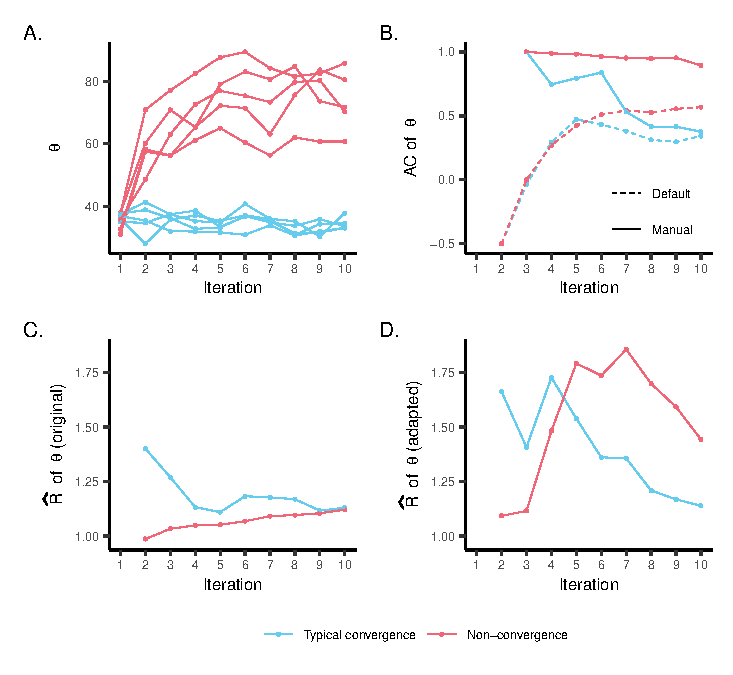
\includegraphics{2.Manuscript_files/figure-latex/diagnostics-1} 

}

\caption{Convergence diagnostics applied on the imputation algorithms of Figure 2. $\theta$ = chain mean in $ \dot y_{\rm imp, \ell} $.}\label{fig:diagnostics}
\end{figure}

\textbf{{[}REPHRASE as active about panel A{]}} From visual inspection, we know that the typically converged algorithm initially portrayed some signs of non-mixing (around \(t=2\)), but intermingled nicely overall. Additionally, there was very little trending. The algorithm with pathological non-convergence showed severe non-mixing, although this gradually improved (from \(t=7\)). In this scenario, there was a lot of trending as well initially (up-to \(t=6\)), after which the chains reached a somewhat more stationary state.

When we look at panel B, we conclude something weird. The \(AC\)-values calculated with the default function indicate equal performance for the typical convergence and the pathological non-convergence (up-to \(t=5\)), while there is obvious trending in the \(\theta\)s of the latter. Moreover, the best convergence (as indicated by the lowest \(AC\)-value) is observed at \(t=2\), but looking at the chain means in panel A, there should be some signs of trending up-to iteration number seven. After consulting the documentation on \texttt{stats::acf()}, we conclude that this \(AC\) function is not suited for iterative imputation algorithms. The function is optimized for performance when \(t\geq50\) \citep{box15}, while the default number of iterations in iterative imputation is often much lower. Therefore, we compute \(AC\) manually, see the solid line. These \(AC\) values indicate non-stationarity as expected. We therefore calculate \(AC\) manually.

\textbf{Describe panel C here and why it is not optimal: NB. In panel C: De grotere variantie overall zorgt er kennelijk voor dat \(\widehat{R}\) groeit. De \(\widehat{R}\) geeft de foutieve boodschap dat convergentie steeds slechter gaat. Verklaring: de overdispersie assumptie klopt niet als er trend is.{]}} The \(\widehat{R}\)-values in panel D do meet the requirements specified above. \(\widehat{R}\) as computed conform \citet{veht19} does indeed indicate less signs of non-convergence as the number of iterations goes up. \textbf{\citep[explain the dip in Rhat values at t=2. Namely, because we can only use 2 of the 3 tricks by][ if the number of iterations is very low (t\textless4). That's why the \(\widehat{R}\)s are more similar to the traditional GR.]{veht19}}

\textbf{In conclusion, we will use \(\widehat{R}\) conform \citet{veht19} and \(AC\) computed manually as non-convergence diagnostics in the simulation study. The diagnostics will be applied to four \(\theta\)s of interest: chain means, chain variances, a quantity of scientific interest, and the first eigenvalue of the variance-covariance matrix. Results in eight methods to identify non-convergence}

\hypertarget{simulation-study}{%
\section{Simulation study}\label{simulation-study}}

The aim of the simulation study is to determine the \textbf{impact of non-convergence {[}``early stopping'' en ``proportion of complete cases''{]}} in iterative imputation algorithms. Specifically, we are interested in the bias and confidence-validity of estimates obtained from incomplete data with the MICE algortihm. \textbf{{[}REMOVE?{]} Subsequently we will evaluate how well \(\widehat{R}\) and \(AC\) perform in identifying the effects of non-convergence }{[}and performance of different thetas{]}\textbf{. And finally, we will formulate an informed advice on the requirements to safely conclude sufficient convergence in practice. That is, we conclude that convergence is sufficient when each estimate \(\bar{Q}\) is an unbiased and confidence-valid estimate of the corresponding estimand \(Q\).}

To induce non-convergence, we consider two sets of simulation conditions: we vary the missingness proportion \(p_{\rm mis}\) in the incomplete data, and we vary the number of iterations \(T\) in the imputation algorithm. The missingness conditions are chosen to reflect the difficulty of the missingness problem. The underlying assumption is that low missingness proportions lead to quick algorithmic convergence, since there is a lot of information in the observed data. Higher missingness proportions should yield slower convergence. Unless, however, the fraction of missing information is so high that the random component in the imputation algorithm outweighs the information in the observed data. Then, convergence to a stable but highly variable state may be reached instantaneously. We expect that the incremental missingness proportions in our study will result in a corresponding increase in signs of non-convergence.

The assumption inherent to the second set of simulation conditions---the number of iterations---is that terminating the imputation algorithm too early causes non-convergence. Generally, the algorithm will not reach convergence if \(T=1\), because the imputed values in the first iteration (at \(t=1\)) depend on the initial values of the algorithm (which are sampled randomly from the set of observed datapoints). As the number of iterations increases, the imputation chains should become independent of the initial values, until the point at which adding an extra iteration does not lead to a more converged state. We assume that we can induce non-convergence at least in conditions where \(T\) is smaller than the default number of iterations in \texttt{mice}, \(T=5\).

\hypertarget{hypotheses}{%
\subsection{Hypotheses}\label{hypotheses}}

\begin{enumerate}
\def\labelenumi{\arabic{enumi}.}
\item
  We expect that simulation conditions with a high missingness proportion \(p_{\rm mis}\) and a low number of iterations \(T\) will more often result in biased, invalid estimates of the quantities of scientific interest, \(Q\)s.
\item
  We hypothesize that \(\widehat{R}\) and \(AC\) will correctly identify signs of non-convergence in those simulation conditions where the \(\bar{Q}\)s are \emph{not} unbiased and confidence-valid estimates of the \(Q\)s.
\item
  We hypothesize that the recommended thresholds to diagnose non-convergence with \(\widehat{R}\) (\(\widehat{R} > 1.2\), \(\widehat{R} > 1.1\), and \(\widehat{R} > 1.01\)) may be too stringent for iterative imputation applications. In an empirical study, where \(\widehat{R}\) was used to inform the required imputation chain length, it took as many as 50 iterations to overcome the conventional non-convergence threshold \(\widehat{R}>1.2\). Yet, scientific estimates were insensitive to continued iteration from \(t=5\) onward \citep{lace07}. We therefore suspect that \(\widehat{R}\) may over-estimate signs of non-convergence in iterative imputation algorithms, compared to the validity of estimates. In contrast to this, it may occur that signs of non-convergence are under-estimated by \(\widehat{R}\), in exceptional cases where the initial values of the algorithm are not appropriately over-dispersed \citep[p.~437]{broo98}. In \texttt{mice}, initial values are chosen randomly from the observed data, hence we cannot be certain of over-dispersion in the initial values. In practice, we do not expect this to cause problems for identifying non-convergence with \(\widehat{R}\). \textbf{{[}ADD limitation that other MI packages may have different way to obtain initial values!{]}}
\item
  We expect that high \(AC\) values are implausible in iterative imputation algorithms with typical convergence. After only a few iterations, the randomness induced by the algorithm should effectively mitigate the risk of dependency within chains.
\item
  We further hypothesize that multivariate \(\theta\)s are better at detecting non-convergence than univariate \(\theta\)s.
\end{enumerate}

\hypertarget{set-up}{%
\subsection{Set-up}\label{set-up}}

We investigate non-convergence of the MICE algorithm through model-based simulation in \texttt{R} \citep[version 3.6.3;][]{R}. The number of simulation repetitions is 1000, and the simulation set-up is summarized in the pseudo-code below. The complete \texttt{R} script of the simulation study is available from \href{https://github.com/gerkovink/shinyMice/tree/master/3.Thesis/}{github.com/gerkovink/shinyMice}.

\begin{verbatim}
# pseudo-code of simulation 
1. simulate data 
for (number of simulation runs from 1 to 1000)
 for (missingness proportions 5%, 25%, 50%, 75% and 95%)
  2. create missingness
  for (number of iterations from 1 to 100)
   3. impute missingness
   4. perform analysis of scientific interest
   5. compute non-convergence diagnostics 
   6. pool results across imputations
   7. compute performance measures
 8. combine outcomes of all missingness proportions
9. aggregate outcomes of all simulation runs 
\end{verbatim}

\hypertarget{data-generating-mechanism.}{%
\subsubsection{Data-generating mechanism.}\label{data-generating-mechanism.}}

In this study, sampling variance is not of interest. Therefore, a single complete dataset may serve as comparative truth in all simulation repetitions \citep{vink14}. The data-generating mechanism is a multivariate normal distribution, representing person-data on three predictor variables in a multiple linear regression problem. Let the predictor space be defined as
\[
\begin{aligned}
\begin{pmatrix}X_1\\
X_2\\
X_3
\end{pmatrix} \sim \mathcal{N}
\begin{bmatrix}
\begin{pmatrix}
12\\
3\\
0.5
\end{pmatrix}\!\!,
\begin{pmatrix}
4 & 4 & 1.8 \\
4 & 16 & 4.8\\
1.8 & 4.8 & 9
\end{pmatrix}
\end{bmatrix}\!\!\text{.}\\[2\jot]
\end{aligned}
\]
A finite population of \(N=1000\) is simulated using the \texttt{mvtnorm} package \citep{mvtnorm}. Subsequently, a fourth variable is constructed as outcome variable \(Y\). For each unit \(i = 1, 2,..., N\), let
\[
Y_i = 1 + 2X_{1i} +.5X_{2i} - X_{3i} + \epsilon_i ,
\]
where \(\epsilon \sim \mathcal{N}(0, 100)\). This results in a complete set \(y\), with observed values for all units \(i\) on all variables \(j\) (where \(j = Y, X_1, X_2, X_3\)). From the complete set we obtain the true values of the scientific estimands \(Q\).

\hypertarget{scientific-estimands.}{%
\subsubsection{Scientific estimands.}\label{scientific-estimands.}}

We consider four types of \(Q\)s that are often of interest in empirical research. Namely, two descriptive statistics: the mean \(\mu_j\) and standard deviation \(\sigma_j\) of each variable \(j\). We also consider the regression coefficients of the predictors: \(\beta_1\), \(\beta_2\), and \(\beta_3\) in regression equation
\[Y' = \beta_0 + \beta_1 X_1 + \beta_2 X_2 + \beta_3 X_3,\]
where \(Y'\) is the expected value of the outcome. And finally, the proportion of variance explained by the set of predictors: coefficient of determination \(r^2\) \textbf{(note that lower case \(r\) is used to avoid confusion with non-convergence diagnostic \(\widehat{R}\))}. These \(Q\)s are estimated by \(\bar{Q}\) in each simulation condition.

\hypertarget{simulation-conditions.}{%
\subsubsection{Simulation conditions.}\label{simulation-conditions.}}

The complete dataset is \emph{amputed} in each simulation repetition to create five incomplete datasets \(y\) with different missingness proportions \(p_{\rm mis}\). The \(p_{\rm mis}\) varies between 5 and 95\%, in incremental steps (\(p_{\rm mis}\) = .05, .25, .50, .75, .95). We consider all possible univariate and multivariate patterns of missingness, conform a `missing completely at random' missingness mechanism \citep{rubin87}. I.e., the probability to be missing is the same for all \(N \times k\) cells in \(y\), conditional on the missingness proportion \(p_{\rm mis}\). This is performed with the `mice' package \citep[function \texttt{mice::ampute()};][]{mice}.

The second set of simulation conditions is the number of iterations in the imputation algorithm. We vary the number of iterations between one and one hundred (\(T = 1,2,.,100\)). All imputation procedures are performed with Bayesian linear regression imputation, and five imputation chains (\(m=5\)). We perform this with the \texttt{mice()} function \citep{mice}. The result is five sets of imputations per simulation condition, \(y_{\rm imp, \ell}\).

Subsequently, we obtain the completed data \{\(y_{\rm obs}, y_{\rm imp, \ell}\)\} by combining the imputed data with the observed data \citep[function \texttt{mice::complete()};][]{mice}. Univariate quantities of scientific interest \(Q\) are estimated directly from the completed data \{\(y_{\rm obs}, y_{\rm imp, \ell}\)\}. Estimates of multivariate \(Q\)s are obtained after employing multiple linear regression \citep[function \texttt{stats::lm()},][]{R}. From the estimates in each imputation, \(\hat{Q}_\ell\), we obtain the pooled estimate \(\bar{Q}\). For univariate estimates we pool \(\hat{Q}_\ell\) as average. Multivariate \(\hat{Q}_\ell\) are pooled conform \citet{vink14}.

\hypertarget{methods.}{%
\subsubsection{Methods.}\label{methods.}}

In total, we consider eight methods to identify non-convergence. Namely, we apply the two non-convergence diagnostics \(\widehat{R}\) and \(AC\) on four different \(\theta\)s. Univariate \(\theta\)s are obtained from \(y_{\rm imp, \ell}\). The multivariate \(\theta\) \(\lambda_{1,\ell}\) is obtained from \{\(y_{\rm obs}, y_{\rm imp, \ell}\)\}. The other multivariate \(\theta\) is equal to the estimated regression coefficient \(\hat{Q}_\ell\) in \{\(y_{\rm obs}, y_{\rm imp, \ell}\)\}. We apply the two non-convergence diagnostics to each \(\theta\) by implementing \citet{veht19} 's recommended \(\widehat{R}\) and we compute \(AC\) manually.

\hypertarget{performance-measures.}{%
\subsubsection{Performance measures.}\label{performance-measures.}}

As recommended by \citet{buur18} we evaluate the performance of the imputation algorithm with bias, coverage rate (CR), and confidence interval width (CIW). Bias is calculated for each \(Q\). CR and CIW only for \(Q = \beta\).
We calculate bias as \(\bar{Q} - Q\). CR is defined as the percentage of simulation repetitions in which the 95\% confidence interval (CI) around \(\bar{Q}\) covers the true estimand \(Q\). Let
\[\text{CI} = \bar{Q} \pm t_{(m-1)} \times \rm SE_{\bar{Q}},\]
where \(t_{(M-1)}\) is the quantile of a \(t\)-distribution with \(m-1\) degrees of freedom, and \(\rm SE_{\bar{Q}}\) is the square root of the pooled variance estimate. If we obtain nominal coverage (CR = 95\%), we can conclude that \(\bar{Q}\) is a confidence-valid estimate of \(Q\). Finally, we inspect CI width (CIW): the difference between the lower and upper bound of the 95\% confidence interval around \(\bar{Q}\). CIW is of interest because it is a measure of efficiency. Under nominal coverage, short CIs are preferred, since wider CIs indicate lower statistical power.

We evaluate the methods to identify non-convergence against these performance measures. \(\widehat{R}\) and \(AC\) should identify non-convergence in simulation conditions, where \(\bar{Q}\) is \emph{not} an unbiased, confidence-valid estimate of \(Q\).

\hypertarget{results}{%
\section{Results}\label{results}}

\textbf{{[}Add more info about figure legends and axes{]}}

Our results show the performance of the MICE algorithm under different conditions of missingness and iteration length. For reasons of brevity, we only discuss results for the worst-performing estimates in terms of bias. For univariate scientific estimands (\(Q=\mu\) and \(Q=\sigma\)) we observe the largest bias in the outcome variable \(Y\). And for the regression coefficients (\(Q=\beta\)) the bias is most pronounced in \(\beta_1\) (the effect of \(X_1\) on \(Y\)). Since there is just one estimate for \(Q=r^2\) to consider, we \textbf{end up with} \(Q=\mu_Y, \sigma_Y,r^2, \beta_1\). In the figures, we present all missingness conditions, but only \textbf{iteration length conditions} \(1 \leq T\leq50\), since the results are more or less stable for conditions where \(T \geq 30\). Full results are available from \href{https://github.com/gerkovink/shinyMice/tree/master/3.Thesis/1.SimulationStudy}{github.com/gerkovink/shinyMice}.

\hypertarget{quantities-of-scientific-interest}{%
\subsection{Quantities of scientific interest}\label{quantities-of-scientific-interest}}

\begin{figure}

{\centering 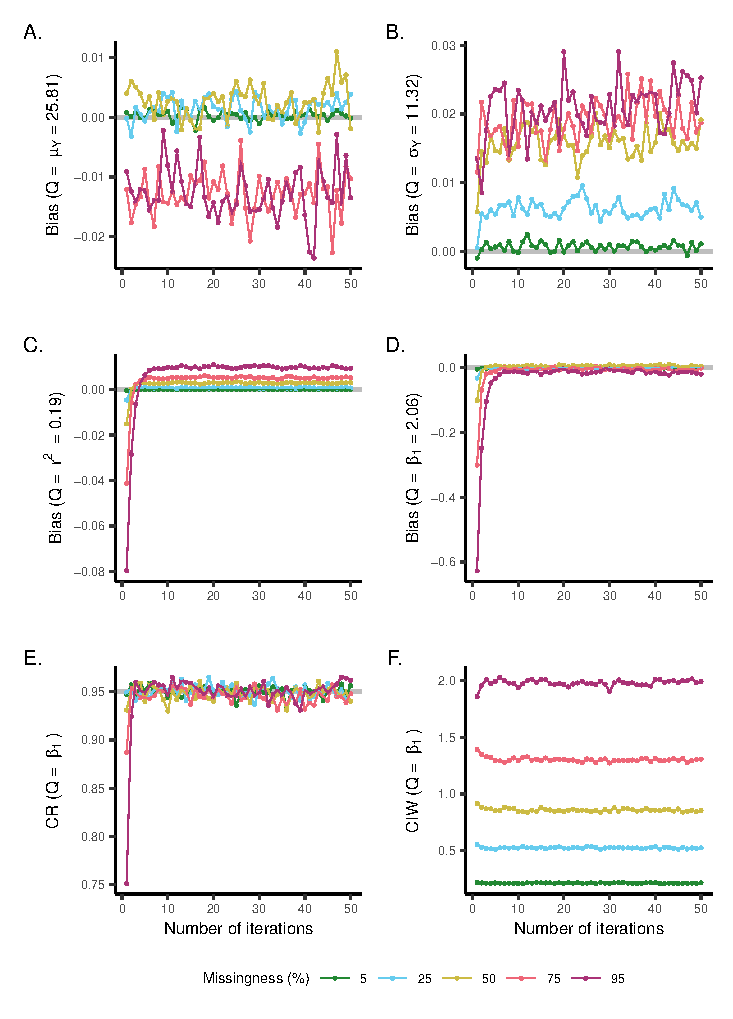
\includegraphics{2.Manuscript_files/figure-latex/Qs-1} 

}

\caption{Impact of non-convergence on statistical inferences. Depicted are the bias, coverage rate (CR) and confidence interval width (CIW) of the estimates $\bar{Q}$. We present the subset of $Q$s with the worst performance in terms of bias: the mean and standard deviation of $Y$, and the regression coefficient of $X_1$.}\label{fig:Qs}
\end{figure}

Figure \ref{fig:Qs} displays the influence of \textbf{inducing non-convergence {[}``early stopping'' en ``proportion of complete cases''{]}} on the estimated quantities of scientific interest, \(Q\)s. \textbf{{[}Add panel labels, describe panels{]}} Simulation conditions that are impacted by non-convergence portray more extreme bias in the estimated \(Q\)s, and non-nominal coverages.

\hypertarget{qmu.}{%
\subsubsection{\texorpdfstring{\(Q=\mu\).}{Q=\textbackslash mu.}}\label{qmu.}}

The estimated univariate means seem unaffected by the number of iterations in the algorithm. This implies that approximately unbiased estimates may be obtained with as little as one iteration (\(T \geq 1\)). The magnitude of the bias in \(\bar{Q}\) depends solely on the missingness proportion \(p_{\rm mis}\), with missingness proportions of 75\% and 95\% leading to more extreme biases than other missingness proportions. Completely unbiased estimates are only obtained in conditions where \(p_{\rm mis}\leq.50\). \textbf{This is curious because the missingness mechanism MCAR should yield unbiased univariate estimates without employing multiple imputation.} Note however, that the magnitude of the bias in these conditions is small: \(\mu_Y\) is maximally under-estimated by 0.02 units, while the true value of \(\mu_Y\) is 25.81 (\(\sigma_Y = 11.32\)). We, therefore, conclude that non-convergence does not substantially impact the validity of the inferences for \(Q=\mu\).

\hypertarget{qsigma.}{%
\subsubsection{\texorpdfstring{\(Q=\sigma\).}{Q=\textbackslash sigma.}}\label{qsigma.}}

The estimated standard deviations not affected substantially by \textbf{early stopping} either. While stable estimates are obtained in conditions with two iterations, the bias in the first iteration is actually \emph{less} severe than in other \textbf{iteration conditions}. Therefore, no iteration at all is needed to obtain approximately unbiased estimates for \(Q=\sigma\). Completely unbiased estimates are only obtained in conditions where \(p_{\rm mis}=.05\). Conditions where \(p_{\rm mis}\geq.25\) are impacted by non-convergence in order of increasing missingness proportion. Similar to the bias for \(Q=\mu\) the magnitude of the bias in \(Q=\sigma\) is negligible. We therefore conclude that neither one of the univariate \(Q\)s is affected substantially by non-convergence.

\hypertarget{qr2.}{%
\subsubsection{\texorpdfstring{\(Q=r^2\).}{Q=r\^{}2.}}\label{qr2.}}

The estimated coefficient of determination is clearly affected by early stopping. As expected, we observe worse performance in conditions with a lower number of iterations. The magnitude of the bias, however, depends on the missingness proportion---following the incremental order in \(p_{\rm mis}\). \textbf{And so does} the number of iterations necessary to reach stable, approximately unbiased estimates. In conditions where \(p_{\rm mis}=.05\), estimates are unbiased after one iteration. We observe approximately unbiased estimates when \(T\geq 2,4, \text{and }5\), in conditions where \(p_{\rm mis} = .25, .50, \text{and }.75\), respectively \textbf{{[}only report the worst?{]}}. The highest number of iterations necessary to reach approximate unbiasedness is seven. Completely unbiased estimates are only obtained in conditions where \(p_{\rm mis}\leq.25\). This implies that even for biased estimates, \(T\geq7\) would suffice to reach a stable solution.

\hypertarget{qbeta.}{%
\subsubsection{\texorpdfstring{\(Q=\beta\).}{Q=\textbackslash beta.}}\label{qbeta.}}

For the estimated regression coefficients, we first consider bias, before discussing CR and CIW. As Figure \ref{fig:Qs} shows, the bias in \(\bar{Q}\) is affected by both the missingness proportion and the number of iterations. Approximately unbiased estimates are observed after one to seven iterations, depending on \(p_{\rm mis}\).Completely unbiased estimates are only obtained in conditions where \(T\geq3\) and \(p_{\rm mis}\leq .50\).

Despite persistant bias in conditions where \(p_{\rm mis}\geq.75\), coverage rates indicate that all \textbf{missingness conditions} have nominal coverages after just three iterations. Confidence-valid estimates may be obtained in any condition where \(T\geq3\).

The nominal coverages are explained by the CIWs. Conform the theoretical foundation of MI, CIs are wider in conditions with higher missingness proportions (i.e., there is less information in the data, and thus more uncertainty due to missingness). The wider CIs around \(\bar{Q}\) in conditions with higher missingness proportions \textbf{results in the inclusion of} the true value of \(Q\) despite of bias.

We conclude that approximately unbiased estimates may be obtained in conditions where \(T\geq7\), whereas confidence-valid estimates require at most three iterations.

\hypertarget{summary}{%
\subsubsection{Summary}\label{summary}}

These results demonstrate that the estimates of univariate scientific estimands \(Q\) are not impacted by early stopping of the MICE algorithm, irrespective of the missingness proportion in \(y\). Unbiased estimates may be obtained after just one iteration. Multivariate estimates, by contrast, are affected by both the number of iterations and the missingness proportion. Completely unbiased estimates are only observed under low to moderate missingness (\(p_{\rm mis}\leq.50\)), after at most three iterations (\(T\leq1,2,3\), depending on \(p_{\rm mis}\)). Approximately unbiased estimates are observed for any missingness condition, after at most seven iterations. This implies that the algorithm produces stable, unimproving estimates for any condition where \(T\geq7\).

\hypertarget{non-convergence-diagnostics-1}{%
\subsection{Non-convergence diagnostics}\label{non-convergence-diagnostics-1}}

Figure \ref{fig:rhats-acs} displays results for the two non-convergence diagnostics applied to the four \(\theta\)s. \textbf{{[}describe panels{]}} We evaluate the performance of these methods by establishing whether they correctly identify conditions in which \(\bar{Q}\) is \emph{not} an unbiased, confidence-valid estimate of \(Q\). Biased estimates are observed in conditions where \(T\leq7\). Non-nominal coverage rates are observed only when \(T\leq3\). Additionally, there is persistant bias in conditions where \(p_{\rm mis}\geq.75\), irrespective of the iteration length. \textbf{{[}appropriate methods thus identify these conditions{]}}

Figure \ref{fig:rhats-acs} displays the non-convergence diagnostics \(\widehat{R}\) and \(AC\) for each of the four \(\theta\)s under consideration. \textbf{{[}Add panel labels and explain how to read the plots{]}}

\begin{figure}

{\centering 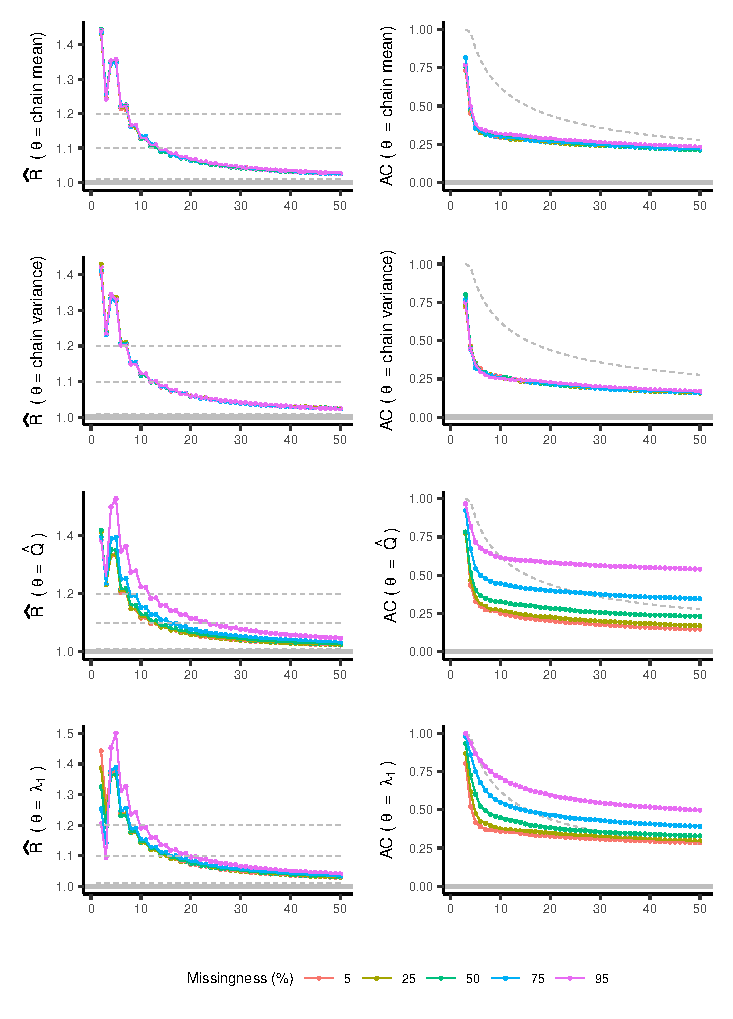
\includegraphics{2.Manuscript_files/figure-latex/rhats-acs-1} 

}

\caption{Non-convergence diagnostics. [Split up into 2 or 4 figures??]}\label{fig:rhats-acs}
\end{figure}

\hypertarget{theta-chain-mean.}{%
\subsubsection{\texorpdfstring{\(\theta=\) chain mean.}{\textbackslash theta= chain mean.}}\label{theta-chain-mean.}}

As expected, \(\widehat{R}\) lowers with the number of iterations. After an initial `dip' in conditions where \(T=3\), we observe a gradual decrease in \(\widehat{R}\)-values with every additional iteration. This implies improving convergence, until the decrease tapers off after 30 to 40 iterations. Using the threshold \(\widehat{R}>1.2\), we diagnose non-convergence in conditions where \(T\leq7\), whereas the threshold 1.1 is exceeded when \(T\leq13\). The very strict threshold 1.01 is surpassed in all conditions \(T\leq100\)\textbf{, and therefore not informative in the current study}. With this method and \(\theta\), we fail to identify simuation conditions with persistant bias due to high missingness proportions.

Similarly, \(AC\) decreases with higher \(T\)s. \(AC\) indicates improving stationarity in conditions where \(T\leq6\). The \(AC\)-values do not exceed the threshold \textbf{defined by statistically significant \(AC\)s}. Based on this threshold, we fail to not diagnose non-convergence in any condition.

\hypertarget{theta-chain-variance.}{%
\subsubsection{\texorpdfstring{\(\theta=\) chain variance.}{\textbackslash theta= chain variance.}}\label{theta-chain-variance.}}

As Figure \ref{fig:rhats-acs} shows, the results of the two diagnostics applied to the chain variances are highly similar to those on the chain means. This holds for both \(\widehat{R}\) and \(AC\). The only apparent difference is in the \(\widehat{R}\) threshold 1.1. Instead of diagnosing non-convergence in conditions where \(T\leq13\), we now diagnose this when \(T\leq11\). All other observations are equivalent.

\hypertarget{thetahatq_ell.}{%
\subsubsection{\texorpdfstring{\(\theta=\hat{Q}_\ell\).}{\textbackslash theta=\textbackslash hat\{Q\}\_\textbackslash ell.}}\label{thetahatq_ell.}}

The \(\widehat{R}\)-values show a similar trend across iterations as we observed for chain means and chain variances. Only conditions with very high missingness proportions (\(p_{\rm mis}\geq.75\)) diverge from the earlier observations. The \(\widehat{R}\)-values in these conditions do not taper off after 30 to 40 iterations, but rather between 40 to 50 iterations. The highest number of iterations at which non-convergence is still diagnosed according to the thresholds are: 11 for \(\widehat{R}>1.2\), 23 for \(\widehat{R}>1.1\), and 100 for \(\widehat{R}>1.01\) \textbf{{[}only report the worst?{]}}.

The \(AC\)-values also follow earlier observations, with the exception of the same very high missingness proportions that \textbf{diverged} for \(\widehat{R}\). To reach maximum stationarity, these conditions require not five but six or seven iterations. Moreover, the \(AC\)-values in these conditions exceed the threshold to diagnose non-convergence. Interestingly, this only occurs after ten or even thrity iterations, while we would expect more signs of trending early in the iterations. \textbf{Since the \(AC\)-values are not improving or worsening after seven iterations, we conclude that non-convergence is incorrectly diagnosed based on the threshold.}

\hypertarget{thetalambda_1-ell.}{%
\subsubsection{\texorpdfstring{\(\theta=\lambda_{1, \ell}\).}{\textbackslash theta=\textbackslash lambda\_\{1, \textbackslash ell\}.}}\label{thetalambda_1-ell.}}

Once again, we observe \(\widehat{R}\)-values with a similar trend across iterations. For this \(\theta\), the results differ only in the most extreme missingness condition. We diagnose non-convergence in conditions where \(T\leq9\) according to \(\widehat{R}>1.2\), and \(T\leq19\) for \(\widehat{R}>1.1\). The `dip' in \(\widehat{R}\)-values at \(T=3\) is even more pronounced than with other \(\theta\)s. Some \(\widehat{R}\)-values even overcome the threshold of 1.2. If we would terminate the algorithm after three iterations, we would incorrectly conclude sufficient convergence according to the \(\widehat{R}>1.2\) threshold.

\(AC\)-values are systematically higher for this \(\theta\) than in the other results. The \(AC\)-values also taper off at a later point in the iterations, indicating improving stationarity up-to ten, or even thirty iterations, depending on the missingness proportion. Using the threashold, we diagnose non-convergence at some point for any missingness proportion.

\hypertarget{summary-1}{%
\subsubsection{Summary}\label{summary-1}}

Overall, the methods to diagnose non-convergence perform as expected: they indicate more signs of non-convergence in conditions with worse performance in terms of bias and confidence-validity. Under low to moderate missingness, it does not seems to matter on which \(\theta\) the diagnostics are applied. If we look at complete unbiasedness, however, we notice that univariate \(\theta\)s fail to diagnose the persistant bias in conditions where \(p_{\rm mis}\geq.75\). The number of iterations necessary to obtain approximately unbiased, confidence-valid estimates corresponds to the \(\widehat{R}\) threshold 1.2. The thresholds 1.1 and 1.01 seem to strict compared to the validity of the inferences. The \(AC\) threshold defined by the statistical significance of the \(AC\)-values does not appear to be appropriate in the current set-up \textbf{{[}or iterative imputation in general??{]}}. Non-stationarity may be better diagnosed by evaluating the \(AC\)-values across iterations. If the values do not substantially decrease, stationarity may be concluded \textbf{{[}similar to the elbow heuristic in PCA{]}}.

\hypertarget{conclusion}{%
\section{Conclusion}\label{conclusion}}

H1: As hypothesized, biased, invalid estimates occur more often in simulation conditions with a higher missingness proportion and lower number of iterations. However, this only holds for multivariate scientific estimands. Univariate \(Q\)s are not substantially impacted by early stopping.

H2: As expected, we observe higher \(\widehat{R}\) and \(AC\)-values in conditions where \(\bar{Q}\)s were biased, invalid estimates of \(Q\)s.

H3: The hypothesis that the recommended thresholds would be too strict is only patially supported. \(\widehat{R}\) indicated improving convergence until 30 to 40 iterations, while approximately unbiased, confidence-valid estimates were obtained after just seven iterations. This rougly corresponds to the threshold of 1.2. The more stringent trheshold 1.1 seems plausible compared to the decrease in \(\widehat{R}\) values across iterations. The most recent threshold 1.01 does indeed seem to over-estimate the signs of non-convergence.

H4: The results of this simulation study do not support the hypothesis that \ldots{} \textbf{{[}insert hypothesis{]}}. We observed \(AC\)-values as high as theoretically possible \(AC=\). The second part of the hypothesis is not refuted: the \(AC\)-values did decrease quicky as a function of \(T\).

H5: We did find some support for the final hypothesis. Multivariate \(\theta\)s indeed have superior performance under certain conditions (e.g., multivariate \(Q\)s and extreme missingness proportions).

\hypertarget{discussion}{%
\section{Discussion}\label{discussion}}

We have shown that non-convergence in iteratiive imputation algorithms leads to biased, invalid estimates of multivariate quantities of scientific interest \(\theta\). Since the current practice of visually inspecting univariate \(\theta\)s does not suffice, we applied non-convergence diagnostics \(\widehat{R}\) and \(AC\) to both univariate and multivariate \(\theta\)s. Signs of non-convergence due to early stopping are identified with each of the methods---i.e., by applying \(\widehat{R}\) and \(AC\) to any \(\theta\). Bias due to high missingness proportions, is only identified with multivariate \(\theta\)s. Under moderate missingness (\(p_{\rm mis}\leq.50\)) \(\widehat{R}\)-values decreased substantially until 30 to 40 iterations, which implies that mixing in the algorithm improved with each additional iteration. \(AC\)-values only improved until about six iterations, suggesting minimal improvement in trending is obtained beyond \(T=6\). Since we obtained approximately unbiased, confidence valid estimates after at most seven iterations, we conclude that the \(\widehat{R}\) threshold 1.2 is the most appropriate diagnostic cut-off. The threshold to diagnose non-stationarity with \(AC\) does not seem to apply. The main finding of this study is that valid inferences may be obtained much quicker than approximate algorithmic convergence is reached. Under the current specifications, univariate \(Q\)s did not require algorithmic convergence at all. They are unbiased almost instantly after the algorithm is initiated. Approximately unbiased, confidence-valid estimates of multivariate \(Q\)s were obtained after a maximum of seven iterations. Continued iterations beyond \(T = 7\) did not yield better estimates.

\hypertarget{implications}{%
\subsection{Implications}\label{implications}}

Iterative imputation algorithms such as MICE have been known to yield valid results under severe missingness. With this study, we have shown that valid inferences can also be obtained under a combination of severe missingness and early stopping. Based on our results, the traditional threshold of \(\widehat{R}> 1.2\) would be appropriate for diagnosing non-convergence in iterative imputation algorithms. This is not in line with the recent recommendations by veht19 to lower the threshold to 1.01. The discrepancy between our conclusion and \citet{veht19}'s may be explained by the nature of iterative imputation algorithms. In the limit, iterative imputation algorithms have the same character as other MCM algorithms, but in imputation procedures a part of the distribution is already determined by the observed data, whereas the entire distribution is unknown in many other MCMC applications. Because we combine a known distribution with an unknown distribution, valid estimates may be reached much sooner. Convergence may therefore be diagnosed at a less stringent threshold. \textbf{{[}HERE were the two asterixes{]}}

The threshold to diagnose non-convergence with \(AC\) does not seem appropriate at all in iterative imputation algorithms. A better diagnostic cut-off would be the number of iterations at which an additional iteration does not substantially decrease \(AC\). In practice, this implies that the default number of iterations in MICE is not sufficient. \(AC\) can only be computed if \(T\geq3\), while the current default in the \texttt{mice} package is five \citep{mice}. Identifying a decrease in the \(AC\)-values across iterations (an `elbow') requires more than three observations. We therefore suggest to increase the default number of iterations in MICE to 10. The computational cost of 5 additional iterations has become less of a burden since MICE was introduced in \citeyearpar{mice}. Moreover, an increased number of iterations would grant the opportunity to exclude the first iterations from evaluation with \(\widehat{R}\). Excluding \(T\leq3\) provides empirical researchers with a less ambiguous heuristic to diagnose non-convergence, because we expect the initial `dip' in \(\widehat{R}\)-values to disappear.

\hypertarget{recommendations-for-empirical-researchers}{%
\subsection{Recommendations for empirical researchers}\label{recommendations-for-empirical-researchers}}

Based on our results, we formulated several recommendations for empirical researchers who employ iterative imputation to draw inferences from incomplete data. We suggest that non-convergence may still be evaluated visually, but in addition to inspecting univariate summaries of the state space of the algorithm (\(\theta\)s, e.g., chain means), multivariate \(\theta\)s should be considered. We propose the following steps:

\begin{enumerate}
\def\labelenumi{\arabic{enumi}.}
\item
  First, check traceplots of the default \(\theta\)s (chain means and chain variances) for signs of pathological non-convergence. Adjust the imputation model if necessary.
\item
  Track multivariate \(\theta\)s over iterations, e.g., the novel \(\theta\) that is scientific model-independent. Or specify your own scalar summary of interest (see e.g., \citet{buur18}). Monitor these \(\theta\)s across iterations through visual inspection, or using a non-convergence diagnostic.
\item
  Compute non-convergence diagnostics \(\widehat{R}\) and \(AC\). Do not use the traditional calculation for \(\widehat{R}\) \citep{gelm92}, or the \texttt{R} function \texttt{stats::acf()} to compute \(AC\) \citep{R}. Instead, calculate \(\widehat{R}\) conform \citet{veht19} and compute autocorrelations manually (see e.g., \href{https://github.com/gerkovink/shinyMice/tree/master/3.Thesis/1.SimulationStudy}{github.com/gerkovink/shinyMice}).
\item
  Use the threshold \(\widehat{R}>1.2\) to diagnose non-mixing, and assess stationarity by plotting the autocorrelation over iterations. Keep iterating until the threshold for mixing is overcome, and until reasonably decreasing asympototic \(AC\)-values are obtained. At that point, inferences are unlikely to improve by continued iteration.
\item
  Profit.
\end{enumerate}

\hypertarget{limitations}{%
\subsection{Limitations}\label{limitations}}

Much remains unknown about non-convergence in iterative imputation algorithms. Even though we have demonstrated the appropriateness of \(\widehat{R}\) and \(AC\) as non-convergence diagnostics in this study, results may not extrapolate to other situations. The current simulation conditions were restricted to a single missingness mechanism. Proper performance under a `missing completely at random' (MCAR) mechanism is a necessary condition for any missing data method. It doesn't, however, guarantee equal performance under different missingness mechanisms. Future research should determine the performance of \(\widehat{R}\) and \(AC\) under `missing at random' and `missing not at random' mechanisms.
Another parameter to consider in future research is the choice of the imputation method. As \citet{murr18} concluded, the behaviour of algorithms such as MICE under certain default imputation models is still an open research question. We have investigated the behaviour of MICE under only one type of model (Bayesian linear regression). Different imputations models might converge more poorly. Moreover, the imputation model may even be mis-specified un purpose to induce different levels of non-convergence. Qualitatively, we have shown that \(\widehat{R}\) and \(AC\) are appropriate under clear violation of convergence. Quantitatively, we have only demonstrated that they can identify signs of non-convergence under MCAR, when the imputation model is a correctly specified Bayesian linear regression model. \newline \newline

\noindent In short, we have shown that an iterative imputation algorithm can yield correct outcomes, even when a converged state has not yet formally been reached. Any further iterations would then burn computational resources without improving the statistical inferences. To conclude, in the case of drawing inference from incomplete data, convergence of the iterative imputation algorithm is often a convenience but not a necessity. \textbf{{[}Our study found that - in the cases considered - inferential validity was achieved after 5-10 iterations, much earlier than indicated by the \(\widehat{R}\) and AC diagnostics. Of course, it never hurts to iterate longer, but such calculations hardly bring added value.{]}}

\bibliographystyle{sageh}
\bibliography{thesis.bib}


\end{document}
